\documentclass{standalone}
\usepackage[utf8]{inputenc}
\usepackage{pgfplots}
\DeclareUnicodeCharacter{2212}{−}
\usepgfplotslibrary{groupplots,dateplot}
\usetikzlibrary{patterns,shapes.arrows}
\pgfplotsset{compat=newest}
\begin{document}
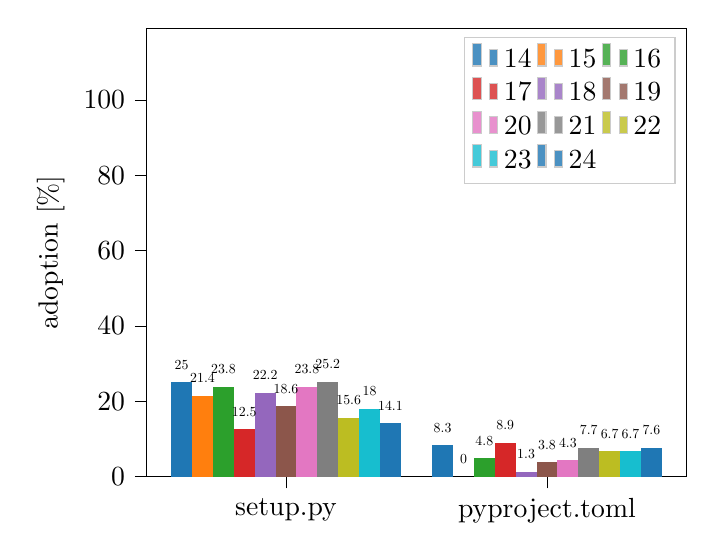
\begin{tikzpicture}

\definecolor{crimson2143940}{RGB}{214,39,40}
\definecolor{darkgray176}{RGB}{176,176,176}
\definecolor{darkorange25512714}{RGB}{255,127,14}
\definecolor{darkturquoise23190207}{RGB}{23,190,207}
\definecolor{forestgreen4416044}{RGB}{44,160,44}
\definecolor{goldenrod18818934}{RGB}{188,189,34}
\definecolor{gray127}{RGB}{127,127,127}
\definecolor{lightgray204}{RGB}{204,204,204}
\definecolor{mediumpurple148103189}{RGB}{148,103,189}
\definecolor{orchid227119194}{RGB}{227,119,194}
\definecolor{sienna1408675}{RGB}{140,86,75}
\definecolor{steelblue31119180}{RGB}{31,119,180}

\begin{axis}[
legend cell align={left},
legend columns=3,
legend style={fill opacity=0.8, draw opacity=1, text opacity=1, draw=lightgray204},
tick align=outside,
tick pos=left,
x grid style={darkgray176},
xmin=-0.454, xmax=1.614,
xtick style={color=black},
xtick={0.08,1.08},
xticklabels={setup.py,pyproject.toml},
y grid style={darkgray176},
ylabel={adoption [\%]},
ymin=0, ymax=119,
ytick style={color=black}
]
\draw[draw=none,fill=steelblue31119180] (axis cs:-0.36,0) rectangle (axis cs:-0.28,25);
\addlegendimage{ybar,ybar legend,draw=none,fill=steelblue31119180}
\addlegendentry{14}

\draw[draw=none,fill=steelblue31119180] (axis cs:0.64,0) rectangle (axis cs:0.72,8.3);
\draw[draw=none,fill=darkorange25512714] (axis cs:-0.28,0) rectangle (axis cs:-0.2,21.4);
\addlegendimage{ybar,ybar legend,draw=none,fill=darkorange25512714}
\addlegendentry{15}

\draw[draw=none,fill=darkorange25512714] (axis cs:0.72,0) rectangle (axis cs:0.8,0);
\draw[draw=none,fill=forestgreen4416044] (axis cs:-0.2,0) rectangle (axis cs:-0.12,23.8);
\addlegendimage{ybar,ybar legend,draw=none,fill=forestgreen4416044}
\addlegendentry{16}

\draw[draw=none,fill=forestgreen4416044] (axis cs:0.8,0) rectangle (axis cs:0.88,4.8);
\draw[draw=none,fill=crimson2143940] (axis cs:-0.12,0) rectangle (axis cs:-0.04,12.5);
\addlegendimage{ybar,ybar legend,draw=none,fill=crimson2143940}
\addlegendentry{17}

\draw[draw=none,fill=crimson2143940] (axis cs:0.88,0) rectangle (axis cs:0.96,8.9);
\draw[draw=none,fill=mediumpurple148103189] (axis cs:-0.04,0) rectangle (axis cs:0.04,22.2);
\addlegendimage{ybar,ybar legend,draw=none,fill=mediumpurple148103189}
\addlegendentry{18}

\draw[draw=none,fill=mediumpurple148103189] (axis cs:0.96,0) rectangle (axis cs:1.04,1.3);
\draw[draw=none,fill=sienna1408675] (axis cs:0.04,0) rectangle (axis cs:0.12,18.6);
\addlegendimage{ybar,ybar legend,draw=none,fill=sienna1408675}
\addlegendentry{19}

\draw[draw=none,fill=sienna1408675] (axis cs:1.04,0) rectangle (axis cs:1.12,3.8);
\draw[draw=none,fill=orchid227119194] (axis cs:0.12,0) rectangle (axis cs:0.2,23.8);
\addlegendimage{ybar,ybar legend,draw=none,fill=orchid227119194}
\addlegendentry{20}

\draw[draw=none,fill=orchid227119194] (axis cs:1.12,0) rectangle (axis cs:1.2,4.3);
\draw[draw=none,fill=gray127] (axis cs:0.2,0) rectangle (axis cs:0.28,25.2);
\addlegendimage{ybar,ybar legend,draw=none,fill=gray127}
\addlegendentry{21}

\draw[draw=none,fill=gray127] (axis cs:1.2,0) rectangle (axis cs:1.28,7.7);
\draw[draw=none,fill=goldenrod18818934] (axis cs:0.28,0) rectangle (axis cs:0.36,15.6);
\addlegendimage{ybar,ybar legend,draw=none,fill=goldenrod18818934}
\addlegendentry{22}

\draw[draw=none,fill=goldenrod18818934] (axis cs:1.28,0) rectangle (axis cs:1.36,6.7);
\draw[draw=none,fill=darkturquoise23190207] (axis cs:0.36,0) rectangle (axis cs:0.44,18);
\addlegendimage{ybar,ybar legend,draw=none,fill=darkturquoise23190207}
\addlegendentry{23}

\draw[draw=none,fill=darkturquoise23190207] (axis cs:1.36,0) rectangle (axis cs:1.44,6.7);
\draw[draw=none,fill=steelblue31119180] (axis cs:0.44,0) rectangle (axis cs:0.52,14.1);
\addlegendimage{ybar,ybar legend,draw=none,fill=steelblue31119180}
\addlegendentry{24}

\draw[draw=none,fill=steelblue31119180] (axis cs:1.44,0) rectangle (axis cs:1.52,7.6);
\draw (axis cs:-0.32,25) ++(0pt,3pt) node[
  scale=0.5,
  anchor=south,
  text=black,
  rotate=0.0
]{25};
\draw (axis cs:0.68,8.3) ++(0pt,3pt) node[
  scale=0.5,
  anchor=south,
  text=black,
  rotate=0.0
]{8.3};
\draw (axis cs:-0.24,21.4) ++(0pt,3pt) node[
  scale=0.5,
  anchor=south,
  text=black,
  rotate=0.0
]{21.4};
\draw (axis cs:0.76,0) ++(0pt,3pt) node[
  scale=0.5,
  anchor=south,
  text=black,
  rotate=0.0
]{0};
\draw (axis cs:-0.16,23.8) ++(0pt,3pt) node[
  scale=0.5,
  anchor=south,
  text=black,
  rotate=0.0
]{23.8};
\draw (axis cs:0.84,4.8) ++(0pt,3pt) node[
  scale=0.5,
  anchor=south,
  text=black,
  rotate=0.0
]{4.8};
\draw (axis cs:-0.08,12.5) ++(0pt,3pt) node[
  scale=0.5,
  anchor=south,
  text=black,
  rotate=0.0
]{12.5};
\draw (axis cs:0.92,8.9) ++(0pt,3pt) node[
  scale=0.5,
  anchor=south,
  text=black,
  rotate=0.0
]{8.9};
\draw (axis cs:0,22.2) ++(0pt,3pt) node[
  scale=0.5,
  anchor=south,
  text=black,
  rotate=0.0
]{22.2};
\draw (axis cs:1,1.3) ++(0pt,3pt) node[
  scale=0.5,
  anchor=south,
  text=black,
  rotate=0.0
]{1.3};
\draw (axis cs:0.08,18.6) ++(0pt,3pt) node[
  scale=0.5,
  anchor=south,
  text=black,
  rotate=0.0
]{18.6};
\draw (axis cs:1.08,3.8) ++(0pt,3pt) node[
  scale=0.5,
  anchor=south,
  text=black,
  rotate=0.0
]{3.8};
\draw (axis cs:0.16,23.8) ++(0pt,3pt) node[
  scale=0.5,
  anchor=south,
  text=black,
  rotate=0.0
]{23.8};
\draw (axis cs:1.16,4.3) ++(0pt,3pt) node[
  scale=0.5,
  anchor=south,
  text=black,
  rotate=0.0
]{4.3};
\draw (axis cs:0.24,25.2) ++(0pt,3pt) node[
  scale=0.5,
  anchor=south,
  text=black,
  rotate=0.0
]{25.2};
\draw (axis cs:1.24,7.7) ++(0pt,3pt) node[
  scale=0.5,
  anchor=south,
  text=black,
  rotate=0.0
]{7.7};
\draw (axis cs:0.32,15.6) ++(0pt,3pt) node[
  scale=0.5,
  anchor=south,
  text=black,
  rotate=0.0
]{15.6};
\draw (axis cs:1.32,6.7) ++(0pt,3pt) node[
  scale=0.5,
  anchor=south,
  text=black,
  rotate=0.0
]{6.7};
\draw (axis cs:0.4,18) ++(0pt,3pt) node[
  scale=0.5,
  anchor=south,
  text=black,
  rotate=0.0
]{18};
\draw (axis cs:1.4,6.7) ++(0pt,3pt) node[
  scale=0.5,
  anchor=south,
  text=black,
  rotate=0.0
]{6.7};
\draw (axis cs:0.48,14.1) ++(0pt,3pt) node[
  scale=0.5,
  anchor=south,
  text=black,
  rotate=0.0
]{14.1};
\draw (axis cs:1.48,7.6) ++(0pt,3pt) node[
  scale=0.5,
  anchor=south,
  text=black,
  rotate=0.0
]{7.6};
\end{axis}

\end{tikzpicture}

\end{document}
